\section{Results}

Main outcome of this report's underlying work is a live application publicly accessible on the Internet. The application hosts the user interface described in the previous section. When opening the URL on the Internet, a map will be shown including a colorful overlay indicating the different clusters for a region. Since the clusters are generated on-the-fly in response to a user query, the overlay is only depicted for a limited region. Figure \ref{fig:eval} shows a sample map including the overlay for Mannheim's city center. The figure summarizes the different pieces of information, the live application is able to provide: The blue points represent various points of interest taken from either the LinkedGeoData or DBPedia databse; and the colorful rectangles display computed clusters. In this case, those results of Mannheim serve as a reference for the evaluation in the following, as team members had the most knowledge about this region. 

Most importantly, the aspect of \textit{meaningfulness} plays a role for the substantial correctness of the application. For this purpose, meaningfulness can be defined as a sensible labelling of clusters. Meaningfulness cannot be formalized; however, cluster labels should be as specific as possible. General terms such that a human could not derive valuable information from it, is to be avoided. According to this definition, the sample result of Mannheim shown in figure \ref{fig:eval} are now to be assessed. Generally, the legend reveals that cluster labels are quite understandable and meaningful to a human. Only the label \textit{shop} leaves room for interpretation. Taking into account the spatial dimension of clusters, the label shop offers potential for  additional criticism. The district \textit{Jungbusch}, known for its lively bar scene. The name shops does not come very close to this information. Likewise, the dataset is very much biased towards schools, i.e. many Mannheim schools are registered in the database, which leads to many datasets getting the label \textit{school}.  Nonetheless, several other clusters provide quite sensible information. The university cluster as well as the touristic cluster in the area of the Mannheimer Wasserturm or even a Universitätsklinikum cluster are  explicitely recognized by the application.

 So, to sum it all up, the application is capable of finding useful information, but heavily depends on the data given in the origin datasets DBPedia and LinkedGeoData.

\begin{figure}
  \centering
    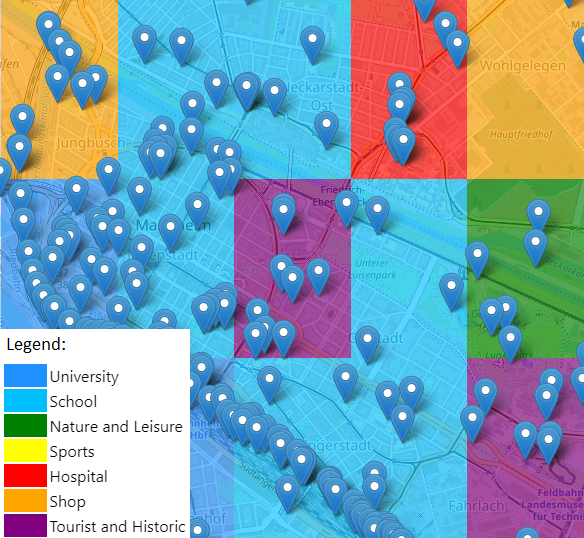
\includegraphics[scale=0.5]{./content/sample.PNG}
  \caption{Evaluation based on sample result in Mannheim}\label{fig:eval}
\end{figure}
